\documentclass[10pt,a4paper]{article}
\usepackage{amsmath}
\usepackage{amssymb}
\usepackage{graphicx}
\usepackage{color}
\usepackage{fancyhdr}
\usepackage{fancyvrb}
\usepackage[margin=3.5cm]{geometry}
\usepackage{framed}
\usepackage{enumerate}
\usepackage{textcomp}
\def\ket#1{\left|#1\right\rangle}
\def\bra#1{\left\langle#1\right|}
\def\braket#1{\left\langle#1\right\rangle}

\definecolor{linkcol}{rgb}{0.0, 0.0, 0.7}
\usepackage[colorlinks=true,urlcolor=linkcol,citecolor=black,linkcolor=linkcol]{hyperref}

\setcounter{section}{0}
\renewcommand\thesection{\arabic{section}}
\renewcommand\thesubsection{\thesection.\arabic{subsection}}

\fancyhf{}
\lhead{\tiny Y.~D.~Chong (2020)}
\rhead{\scriptsize MH2801: Complex Methods for the Sciences}
\lfoot{}
\rfoot{\thepage}
\pagestyle{fancy}

\begin{document}
\setcounter{page}{7}

\section{Derivatives}\label{derivatives}

The \textbf{derivative} of a function $f$ is another function, $f'$,
defined as
\begin{align}
  f'(x) \;\equiv\; \frac{df}{dx} \;\equiv\; \lim_{\delta x \rightarrow 0} \, \frac{f(x + \delta x) - f(x)}{\delta x}.
\end{align}
This kind of expression is called a \textbf{limit expression} because
it involves a limit (in this case, the limit $\delta x \rightarrow
0$).

If the derivative exists (i.e., the above limit expression is
well-defined) over some domain of $x$, we say that $f$ is
\textbf{differentiable} in that domain.  It can be shown that a
differentiable function is automatically continuous.

If $f$ is differentiable, we can define its second-order derivative
$f''$ as the derivative of $f'$. Third-order and higher-order
derivatives are defined similarly.

Graphically, the derivative represents the slope of the graph of
$f(x)$, as shown in the figure below.  The second derivative
represents the curvature; in this figure, the curve is upward-curving
so the second derivative is positive.

\begin{figure}[h]
  \centering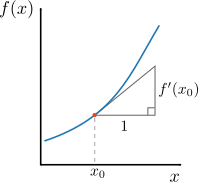
\includegraphics[width=0.32\textwidth]{derivative}
\end{figure}

\subsection{Properties of derivatives}
\label{properties-of-derivatives}

\subsubsection{Rules for limit expressions}
\label{rules-for-limit-expressions}

Let us briefly review the mathematical rules governing limit expressions.

First, the limit of a linear superposition is equal to the linear
superposition of limits. Given two constants $a_1$ and $a_2$ and two
functions $f_1$ and $f_2$,
\begin{align}
  \lim_{x \rightarrow c} \big[a_1 \,f_1(x) \;+\; a_2\, f_2(x)\big] = a_1 \lim_{x \rightarrow c} f_1(x) \;+\; a_2 \lim_{x \rightarrow c} f_2(x).
\end{align}
Second, limits obey a product rule and a quotient rule:
\begin{align}
  \lim_{x \rightarrow c} \big[\;f_1(x) \; f_2(x)\;\big] &= \Big[\lim_{x \rightarrow c} f_1(x)\Big]\;\Big[\lim_{x \rightarrow c} f_2(x)\Big]
  \\ \lim_{x \rightarrow c} \left[\;\frac{f_1(x)}{f_2(x)}\;\right] &= \frac{\lim_{x \rightarrow c} f_1(x)}{\lim_{x \rightarrow c} f_2(x)}.
\end{align}
As a special exception, the product rule and quotient rule are
inapplicable if they result in $0 \times \infty$, $\infty/\infty$, or
$0/0$, which are undefined. As an example of why such combinations are
problematic, consider this:
\begin{align*}
  \lim_{x \rightarrow 0} \;x = \lim_{x \rightarrow 0}\Big[\,x^2\;\frac{1}{x}\;\Big] \overset{?}{=} \lim_{x \rightarrow 0}\Big[\,x^2\,\Big]\; \lim_{x \rightarrow 0}\Big[\,\frac{1}{x}\,\Big] = 0 \, \times \, \infty \;\;(??)
\end{align*}
In fact, the true value of the limit expression is 0; the second step
was incorrect, since it involved an attempt to apply the product rule
where it is inapplicable.

\subsubsection{Composition rules for derivatives}
\label{composition-rules-for-derivatives}

Using the rules for limit expressions, we can derive the following
elementary composition rules for derivatives:
\begin{align}
  \frac{d}{dx}\big[\,\alpha\, f(x) + \beta\, g(x)\,\big] &= \alpha\, f'(x) + \beta\, g'(x) \quad &\textrm{(linearity)}& \\   \frac{d}{dx}\big[\,f(x) \, g(x)\,\big] &= f(x) \, g'(x) + f'(x) \, g(x) &\textrm{(product}\;\textrm{rule)}& \\   \frac{d}{dx}\big[\,f(g(x))\,\big] &= f'(g(x)) \, g'(x) &\textrm{(chain}\;\textrm{rule)}&
\end{align}
These can all be proven by direct substitution into the definition of
the derivative, and taking appropriate orders of limits.  With the aid
of these rules, we can prove various standard results, such as the
``power rule'' for derivatives:
\begin{align}
  \frac{d}{dx} \big[x^n\big] = n x^{n-1}, \;\;n \in \mathbb{N}.
\end{align}
Moreover, the linearity of the derivative operation implies that
derivatives ``commute'' with sums, i.e. you can move them to the left
or right of summation signs. This is a very useful feature. For
example, we can use it to prove that the exponential is its own
derivative, as follows:
\begin{align}
  \frac{d}{dx} \left[\exp(x)\right] &= \frac{d}{dx} \sum_{n=0}^\infty\frac{x^n}{n!} \\
  &= \sum_{n=0}^\infty\frac{d}{dx} \, \frac{x^n}{n!} \\
  &= \sum_{n=1}^\infty \frac{x^{n-1}}{(n-1)!} \\
  &=\exp(x).
\end{align}

Derivatives also commute with limits.  For example, we can use this to
prove that the exponential is its own derivative, using the
alternative definition of the exponential function discussed in
Exercise 1 of Chapter 0:
\begin{align}
  \frac{d}{dx} \left[\exp(x)\right] &= \frac{d}{dx} \lim_{n\rightarrow\infty} \left(1+\frac{x}{n}\right)^n \\
  &= \lim_{n\rightarrow\infty} \frac{d}{dx} \left(1+\frac{x}{n}\right)^n \\
  &= \lim_{n\rightarrow\infty} \left(1+\frac{x}{n}\right)^{n-1} \\
  &= \exp(x).
\end{align}

\subsection{Taylor series}\label{taylor-series}

A function is \textbf{infinitely differentiable} at a point $x_0$ if
all orders of derivatives (i.e., the first derivative, the second
derivative, etc.) are well-defined at $x_0$. If a function is
infinitely differentiable at $x_0$, then near that point it can be
expanded in a \textbf{Taylor series}:
\begin{align}
  f(x) \;&\leftrightarrow\; \sum_{n=0}^\infty \frac{(x-x_0)^n}{n!} \left[\frac{d^nf}{dx^n}\right](x_0) \\
  &=\; f(x_0) + (x-x_0)\, f'(x_0) + \frac{1}{2}\, (x-x_0)^2\, f''(x_0) + \cdots
\end{align}
Here, the ``zeroth derivative'' refers to the function itself. The
Taylor series can be derived by assuming that $f(x)$ can be written as
a general polynomial involving terms of the form $(x-x_0)^n$, and then
using the definition of the derivative to find the series
coefficients.

Here are some common Taylor series:
\begin{align}
  \frac{1}{1-x} &= 1 + x + x^2 + x^3 + \cdots
  \qquad\quad \mathrm{for} \; |x| < 1  \\
  \ln(1-x) &= -x - \frac{x^2}{2} - \frac{x^3}{3} - \frac{x^4}{4} - \cdots \quad \mathrm{for} \; |x| < 1 \\
  \sin(x) &= x - \frac{x^3}{3!} + \frac{x^5}{5!} - \frac{x^7}{7!} + \cdots
  \label{sin_taylor} \\
  \cos(x) &= 1 - \frac{x^2}{2!} + \frac{x^4}{4!} - \frac{x^6}{6!} + \cdots
  \label{cos_taylor} \\
  \exp(x) &= 1 + x + \frac{x^2}{2!} + \frac{x^3}{3!} + \cdots
  \label{exp_taylor} \\
  \sinh(x) &= x + \frac{x^3}{3!} + \frac{x^5}{5!} + \frac{x^7}{7!} + \cdots \\
  \cosh(x) &= 1 + \frac{x^2}{2!} + \frac{x^4}{4!} + \frac{x^6}{6!} + \cdots
  \label{cosh_taylor}
\end{align}
Note that it is possible for a function to have a divergent Taylor
series, or a Taylor series that converges to a different value than
the function itself. The conditions under which such breakdowns occur
is a complicated topic that we will not delve into.

For certain functions, however, the Taylor series are exact. The
Taylor series for the exponential, Eq.~\eqref{exp_taylor}, is exactly
the same as the definition of the exponential itself. Likewise, for
Eqs.~\eqref{sin_taylor}--\eqref{cosh_taylor}, the Taylor series can be
shown to converge to the value of the function for all
$x\in\mathbb{R}$, which means that the series form is \textit{exactly
  equivalent} to the function itself. (Thanks to this, it is common
for math textbooks to start out by \textit{defining} the trigonometic
functions in series form, and then deriving their geometric meanings,
rather than vice versa.)

\subsection{Ordinary differential equations}
\label{ordinary-differential-equations}

Differential equations are equations that contain derivatives.  For
example, the equation
\begin{align}
  \frac{df}{dx} = f(x)
\end{align}
involves both $f$ and its first derivative. It is called an
\textbf{ordinary differential equation}, meaning that it contains a
derivative with respect to a single variable $x$, rather than multiple
variables.

Solving a differential equation means finding a function that
satisfies the equation. There is no single method for solving
differential equations.  Sometimes, we can guess the solution; for
example, by trying different elementary functions, we can discover
that the above differential equation is solved by
\begin{align}
  f(x) = A \exp(x).
\end{align}
Certain classes of differential equation can be solved using
techniques like Fourier transforms, Green's functions, etc., some of
which will be taught in this course. On the other hand, many
differential equations have no known exact analytic solution.

\clearpage

\begin{framed}\noindent
  \textit{Example}---The following ordinary differential equation
  describes a damped harmonic oscillator:
  \begin{align}
    \frac{d^2 x}{dt^2} + 2\gamma\frac{dx}{dt} + \omega_0^2 x(t) = 0.
    \label{eq:dho}
  \end{align}
  In this case, $x(t)$ is the function, and $t$ is the input
  variable. This is unlike our previous notation where $x$ was the
  input variable, so don't get confused! This equation is obtained by
  applying Newton's second law to an object moving in one dimension,
  subject to both a damping force and a restoring force, with $x(t)$
  denoting the position as a function of time $t$.  We will study
  Eq.~\eqref{eq:dho} in detail later in the course.
\end{framed}

\subsubsection{Specific solutions and general solutions}
\label{specific-solutions-and-general-solutions}

When confronted with an ordinary differential equation, the first
thing you should check is the highest derivative appearing in the
equation.  This is called the \textbf{order} of the differential
equation.  If the equation has order $N$, its \textbf{general
  solution} contains $N$ \textbf{free parameters} that can be assigned
any value. Therefore, if you happen to guess a solution, but that
solution does not contain $N$ free parameters, then you know the
solution isn't the most general one.

For example, the ordinary differential equation
\begin{align}
  \frac{df}{dx} = f(x)
\end{align}
has order one. We have previously guessed the solution $f(x) = A
\exp(x)$, which has one free parameter, $A$.  So we know our work is
done: there is no solution more general than the one we found.

A \textbf{specific solution} to a differential equation is a solution
containing no free parameters.  One way to get a specific solution is
to start from a general solution, and assign a value to every free
parameter. In physics problems, the assigned values are commonly
determined by \textbf{boundary conditions}. For an ordinary
differential equation of order $N$, we need independent boundary $N$
conditions to define a specific solution.

\subsection{Partial derivatives}
\label{partial-derivatives}

So far, we have focused on functions which take a single
input. Functions can also take multiple inputs; for instance, we can
have a function $f$ that takes two input numbers, $x$ and $y$, and
outputs a number $f(x,y)$. We can define a \textbf{partial derivative}
as a derivative of a function with respect to one of the inputs,
keeping all other inputs fixed.

For example, the function
\begin{align}
  f(x,y) = \sin(2x - 3 y^2)
\end{align}
has the following partial derivatives:
\begin{align}
  \frac{\partial f}{\partial x} = 2\cos(2x-3y^2), \quad
  \frac{\partial f}{\partial y} = - 6\cos(2x-3y^2).
\end{align}

\subsubsection{Change of variables}
\label{change-of-variables}

We saw in Section~\ref{composition-rules-for-derivatives} that
single-variable functions obey a derivative composition rule,
\begin{align}
  \frac{d}{dx}\, f\big(g(x)\big) = g'(x) \, f'\big(g(x)\big).
\end{align}
This composition rule can be generalized to partial derivatives, which
is often required when performing a \textbf{change of
  coordinates}. Suppose we have a function $f(x,y)$, and we want to
re-express $(x, y)$ in a different coordinate system $(u, v)$. Each
coordinate in the old system may depend on \textit{both} coordinates
in the new system:
\begin{align}
  x = x(u,v), \quad y = y(u,v).
\end{align}
Expressed in the new coordinates, the function is
\begin{align}
  F(u,v) \equiv f\big(x(u,v), y(u,v)\big).
\end{align}
It can be shown that the transformed function's partial derivatives
obey the composition rule
\begin{align}
  \frac{\partial F}{\partial u} &= \frac{\partial f}{\partial x} \frac{\partial x}{\partial u} + \frac{\partial f}{\partial y} \frac{\partial y}{\partial u}\\
  \frac{\partial F}{\partial v} &= \frac{\partial f}{\partial x} \frac{\partial x}{\partial v} + \frac{\partial f}{\partial y} \frac{\partial y}{\partial v}.
\end{align}
On the right-hand side of these equations, the partial derivatives are
meant to be expressed in terms of the new coordinates $(u,v)$.  For
example,
\begin{align*}
  \frac{\partial f}{\partial x} \equiv \left.\frac{\partial f}{\partial x}\right|_{x = x(u,v), \;y= y(u,v)}
\end{align*}

The generalization of this rule to more than two inputs is
straightforward.  For a function $f(x_1, \dots, x_N)$, a change of
coordinates $x_i = x_i(u_1, \dots, u_N)$ involves the composition
\begin{align}
  F(u_1, \dots, u_N) &= f\big(x_1(u_1,\dots,u_N\big), \dots\big), \\
  \frac{\partial F}{\partial u_i} &= \sum_{j=1}^N \frac{\partial f}{\partial x_j}\, \frac{\partial x_j}{\partial u_i}.
\end{align}

\begin{framed}\noindent
  \textit{Example}---In two dimensions, Cartesian and polar coordinates are related by
  \begin{align}
    x = r\cos\theta, \quad y = r\sin\theta.
  \end{align}
  Given a function $f(x,y)$, we can re-write it in polar coordinates
  as $F(r,\theta)$. The partial derivatives in polar coordinates are
  then given by
  \begin{align}
    \frac{\partial F}{\partial r} &= \frac{\partial f}{\partial x} \frac{\partial x}{\partial r} + \frac{\partial f}{\partial y} \frac{\partial y}{\partial r} = \frac{\partial f}{\partial x} \cos\theta + \frac{\partial f}{\partial y} \sin\theta. \\
    \frac{\partial F}{\partial \theta} &= \frac{\partial f}{\partial x} \frac{\partial x}{\partial \theta} + \frac{\partial f}{\partial y} \frac{\partial y}{\partial \theta} = -\frac{\partial f}{\partial x} r\,\sin\theta + \frac{\partial f}{\partial y} r\cos\theta.
  \end{align}
\end{framed}


\subsubsection{Partial differential equations}
\label{partial-differential-equations}

A \textbf{partial differential equation} is a differential equation
involving multiple partial derivatives (as opposed to an ordinary
differential equation, which involves derivatives with respect to a
single variable).

An example of a partial differential equation encountered in physics
is Laplace's equation,
\begin{align}
  \frac{\partial^2 \Phi}{\partial x^2} + \frac{\partial^2 \Phi}{\partial y^2} + \frac{\partial^2 \Phi}{\partial z^2}= 0,
\end{align}
which describes the electrostatic potential $\Phi(x,y,z)$ at position
$(x,y,z)$, in the absence of any electric charges.

Partial differential equations are considerably harder to solve than
ordinary differential equations.  In particular, their boundary
conditions are more complicated to specify: whereas each boundary
condition for an ordinary differential equation consists of a single
number (e.g., the value of $f(x)$ at some point $x = x_0$), each
boundary condition for a partial differential equation consists of a
\textit{function} (e.g., the values of $\Phi(x,y,z)$ along some curve
$g(x,y,z) = 0$).

\subsection{Exercises}\label{exercises}

\begin{enumerate}
\item
  Show that if a function is differentiable, then it is also
  continuous.

\item
  Prove that the derivative of $\ln(x)$ is $1/x$.
  \hfill{\scriptsize [solution~available]}

\item
  Using the definition of non-natural powers, prove that
  \begin{equation}
    \frac{d}{dx} [x^y] = y x^{y-1},
    \quad\mathrm{for}\;\;x \in \mathbb{R}^+, \; y \notin \mathbb{N}.
  \end{equation}

\item
  Consider $f(x) = \tanh(\alpha x)$.

  \begin{enumerate}[(a)]
  \item
    Sketch $f(x)$ versus $x$, for two cases: (i) $\alpha = 1$ and
    (ii) $\alpha \gg 1$.

  \item
    Sketch the derivative function $f'(x)$ for the two cases, based on
    your sketches in part (A) (i.e., without evaluating the derivative
    directly).

  \item
    Evaluate the derivative function, and verify that the result matches
    your sketches in part (B).
  \end{enumerate}

\item
  Prove geometrically that the derivatives of the sine and cosine
  functions are:
  \begin{equation}
    \frac{d}{dx}\sin(x) = \cos(x), \quad\frac{d}{dx}\cos(x) = -\sin(x).
  \end{equation}
  Hence, derive their Taylor series, Eqs.~\eqref{sin_taylor} and
  \eqref{sin_taylor}.

\item
  For each of the following functions, derive the Taylor series around
  $x = 0$:

  \begin{enumerate}[(a)]
  \item
    $f(x) = \ln\left[\alpha \cos(x)\right]$, to the first 3
    non-vanishing terms.

  \item
    $f(x) = \cos\left[\pi\exp(x)\right]$, to the first 4 non-vanishing
    terms.

  \item
    $\displaystyle f(x) = \frac{1}{\sqrt{1 \pm x}}$, to the first 4
    non-vanishing terms. Keep track of the signs (i.e., $\pm$ versus
    $\mp$).
  \end{enumerate}

\item
  For each of the following functions, sketch the graph and state the
  domains over which the function is differentiable:

  \begin{enumerate}[(a)]
  \item
    $f(x) = |\sin(x)|$

  \item
    $f(x) = \left[\tan(x)\right]^2$

  \item
    $\displaystyle f(x) = \frac{1}{1-x^2}$
  \end{enumerate}

\item
  Let $\vec{v}(x)$ be a \emph{vectorial} function which takes an input
  $x$ (a number), and gives an output value $\vec{v}$ that is a
  2-component vector. The derivative of this vectorial function is
  defined in terms of the derivatives of each vector component:
  \begin{equation}
    \vec{v}(x) = \begin{bmatrix}v_1(x) \\ v_2(x)\end{bmatrix}
    \;\; \Rightarrow \;\; \frac{d\vec{v}}{dx} = \begin{bmatrix}dv_1/dx \\
      dv_2/dx\end{bmatrix}.
  \end{equation}
  Now suppose $\vec{v}(x)$ obeys the vectorial differential equation
  \begin{equation}
    \frac{d\vec{v}}{dx} = \mathbf{A} \vec{v},
  \end{equation}
  where
  \begin{equation}
    \mathbf{A} = \begin{bmatrix}A_{11} & A_{12} \\ A_{21} & A_{22}\end{bmatrix}
  \end{equation}
  is a matrix that has two distinct real eigenvectors with real
  eigenvalues.

  \begin{enumerate}[(a)]
  \item
    How many independent numbers do we need to specify for the general
    solution?

  \item
    Let $\vec{u}$ be one of the eigenvectors of $\mathbf{A}$, with
    eigenvalue $\lambda$:
    \begin{equation}
      \mathbf{A} \vec{u} = \lambda \vec{u}.
    \end{equation}
    Show that $\vec{v}(x) = \vec{u}\, e^{\lambda x}$ is a specific
    solution to the vectorial differential equation. Hence, find the
    general solution.
  \end{enumerate}
  \vskip -0.1in
  \hfill{\scriptsize [solution~available]}

\end{enumerate}


    % Add a bibliography block to the postdoc
    
    

\end{document}
